\newpage
\section[Day 4: Cauchy-Schwarz and Euclidean Spaces]{Euclidean Spaces}





\subsection{Euclidean Spaces}

	For each positive integer k, let $\mathbb{R}$$^\text{k}$ be the set of all ordered k-tuples:

	\qquad x = $(x_1,...,x_k)$	\qquad \qquad for each $x_i$ $\in$ $\mathbb{R}$

	with the properties:
	\begin{itemize}[leftmargin=1cm, itemsep=0.4em]
		\item x+y = $(x_1+y_1,...,x_k+y_k)$ $\in$ $\mathbb{R}^{\text{k}}$
	
		\item cx = $(cx_1,...,cx_k)$ $\in$ $\mathbb{R}$$^\text{k}$
	\end{itemize}

	So, $\mathbb{R}$$^\text{n}$ has a vector space structure. Similarly, for $\mathbb{C}^{\text{n}}$. \\


{ \color{blue} Definition 4.1.1: Inner Product for $\mathbb{R}^k$} 

	\qquad $x \cdot y = x_1y_1 + ... + x_ky_k$ $\in$ $\mathbb{R}$ \\

{ \color{blue} Definition 4.1.2: Norm }

	\qquad $|x| = \sqrt{x \cdot x}$ = $\sqrt{\sum_{i=1}^n x_i^2}$ \\

{ \color{blue} Definition 4.1.3: Extension to $\mathbb{C}^k$ } 

	\qquad For z,w $\in$ $\mathbb{C}^n$
	\begin{itemize}[leftmargin=2cm, itemsep=0.4em]
		\item $z \cdot w = z_1\overline{w_1} + ... + z_k\overline{w_k}$
	
		\item $z \cdot z = z_1\overline{z_1} + ... + z_k\overline{z_k}
			= |z_1|^2 + ... + |z_n|^2$ = $|z|^2$
	\end{itemize}





\subsection{Cauchy-Schwarz} 

{ \color{red} Theorem 4.2.1: Cauchy-Schwarz } 

	\qquad If $\alpha_1 , ... , \alpha_n$ $\in$ $\mathbb{C}$ and $b_1 , ... , b_n$ $\in$
	$\mathbb{C}$, then:

	\qquad \qquad $| \sum_{\text{j=1}}^{n} a_j(\overline{b_j})  |^2 \leq
	\sum_{\text{j=1}}^{n} |a_j|^2 \sum_{\text{j=1}}^{n} |b_j|^2 $

{ \color{magenta} \underline{Proof} } 

	Let $A = \sum$ $|a_j|^2$ and $B = \sum$ $|b_j|^2$ and $C = \sum$ $a_j(\overline{b_j})$.

	If $B = 0$, then $b_1$ = ... = $b_n$ = 0. Thus, $0 \leq A(0)$ holds true.

	Suppose $B > 0$. Then:

	\qquad $\sum$ $|Ba_j - Cb_j|^2$ = $\sum$ $(Ba_j - Cb_j)\overline{(Ba_j - Cb_j)}$
	= $\sum$ $(Ba_j - Cb_j)(\overline{B} \ \overline{a_j} - \overline{C} \ \overline{b_j})$

	\qquad = $\sum$ $(Ba_j-Cb_j)(B\overline{a_j}-\overline{C} \ \overline{b_j})$
	= $\sum$ $B^2a_j\overline{a_j} - B\overline{C}a_j\overline{b_j} - BC\overline{a_j}b_j
	+ C\overline{C}b_j\overline{b_j}$

		\qquad = $B^2 \sum |a_j|^2 - B\overline{C}\sum a_j\overline{b_j}
	- BC \sum \overline{a_j}b_j+ |C|^2 \sum |b_j|^2$

	\qquad = $B^2A - B\overline{C}C - BC\overline{C} + |C|^2B$
	= $B^2A - 2|C|^2B + |C|^2B$ = $B^2A -|C|^2B$

	\qquad = $B(AB - |C|^2)$

	Since $| Ba_j - Cb_j |$ $\geq$ 0, then $B(AB - |C|^2)$ $\geq$ 0.

	Since $B$ $>$ 0, then $AB - |C|^2$ $\geq$ 0 so $AB$ $\geq$ $|C|^2$. \\

{ \color{blue} Definition 4.2.2: Consequence of the Cauchy-Schwarz } 

	Since $|z_i|^2 = z_i\overline{z_i}$, then
	$\sum z_i\overline{z_i} = \sum |z_i|^2$ = $|z|^2$. Thus:

	\qquad $|z \cdot w|^2$ = $|\sum z_i\overline{w_i} \ |^2$
	$\leq$ $\sum |z_i|^2 \sum |w_i|^2$ = $|z|^2$ $|w|^2$
	
	Thus, $|z \cdot w|$ $\leq$ $|z| |w|$.

\newpage

{ \color{blue} Propositions 4.2.3 } 

	\qquad Let $x,y,z$ $\in$ $\mathbb{R}^k$ where $\alpha$ $\in$ $\mathbb{R}$:
	\begin{enumerate}[label=(\alph*), leftmargin=2cm, itemsep=0.4em]
		\item $|x|$ $\geq$ 0 where $|x| = 0$ only if x = 0

			{ \color{magenta} \underline{Proof} } 
		
				$|x| = \sqrt{\sum_{i=1}^{k} x_i^2} \geq 0$ where $|x| = 0$ only if $x_1 = ... = x_k = 0$ 

		\item $|\alpha x|$ = $|\alpha| |x|$

			{ \color{magenta} \underline{Proof} } 
		
				$|\alpha x|$ = $\sqrt{\sum_{i=1}^k (\alpha x_i)^2}$
				= $\sqrt{\alpha^2} \sqrt{\sum_{i=1}^k x_i^2}$ = $|\alpha| |x|$
	
		\item $|x+y|$ $\leq$ $|x| + |y|$

			{ \color{magenta} \underline{Proof} } 
		
				$|x+y|^2$ = $(x+y) \cdot (x+y)$ = $|x|^2 + 2(x \cdot y) + |y|^2$

				$\leq$ $|x|^2 + 2|x||y| + |y|^2$ = $(|x|+|y|)^2$

		\item $|x-y|$ $\leq$ $|x-z| + |y-z|$

			{ \color{magenta} \underline{Proof} } 
		
				$|x-y|$ = $|x-z + z-y|$ $\leq$ $|x-z| + |z-y|$ = $|x-z| + |y-z|$
	\end{enumerate}





\subsection{Cardinality}

{ \color{blue} Definition 4.3.1: Onto and 1-1 Mapping } 

	\begin{adjustbox}{minipage=14cm, right, vspace=0.1cm 0cm}
		Suppose for every x $\in$ A, there is an associated f(x) $\in$ B.

		Then f maps A into B = f: A $\rightarrow$ B.
		\begin{itemize}[leftmargin=1cm, itemsep=0.4em]
			\item If f(A) = B, then f maps A onto B.
			
			\item If for each y $\in$ B, f$^{-1}$(y) consist of at most one x $\in$ A
				where f$^{-1}$(y$_1$) = x$_1$ $\neq$ x$_2$ = f$^{-1}$(y$_2$) for y$_1$ $\neq$ y$_2$,
				then f is a 1-1 mapping of A into B.
		\end{itemize}
	\end{adjustbox}

\begin{figure}[h]
	\centering
	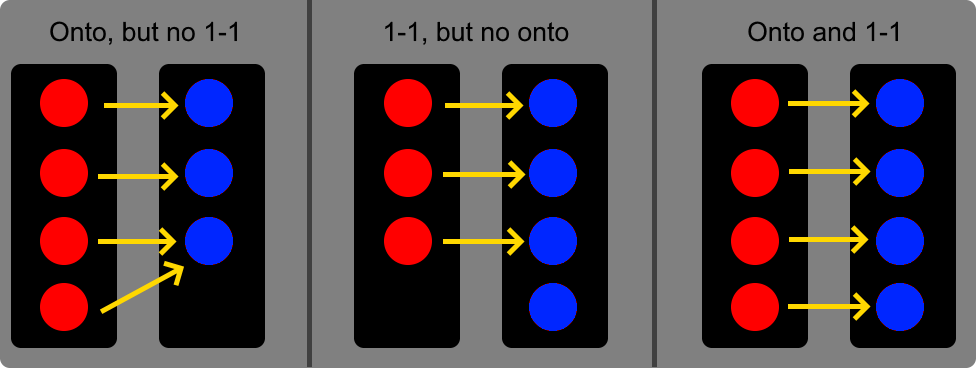
\includegraphics[scale=0.3]{Images/4.3.1.png}
\end{figure}

{ \color{blue} Definition  4.3.2: 1-1 Correspondence} 

	\begin{adjustbox}{minipage=14cm, right, vspace=0.1cm 0cm}
		Sets A and B are equivalent {\color{lblue} (have the same cardinality)} if there is
		a 1-1 onto function f: A $\rightarrow$ B. {\color{lblue} (1-1 correspondence between A and B)}
		Then:

		\qquad A $\sim$ B

		If f: A $\rightarrow$ B is 1-1 and onto, then
		there is a f$^{-1}$: B $\rightarrow$ A that is 1-1 and onto. \\
	\end{adjustbox}

{ \color{blue} Definition 4.3.3: Countability } 
	\begin{itemize}[leftmargin=1cm, itemsep=0.4em]
		\item A is {\color{lblue} finite} if A $\sim$ J$_n$ = \{0, 1, ..., n\}
			for some n $\in$ $\mathbb{N}$
		\item A is {\color{lblue} infinite} if A is not finite
		\item A is {\color{lblue} countably infinite} if A $\sim$ $\mathbb{Z}_+$ = J
		\item A is {\color{lblue} uncountable} if A is not finite or countably infinite
		\item A is {\color{lblue} at most countable} if A is finite or countably infinite. \\
	\end{itemize}

\newpage

{ \color{purple} Example 4.3.4 } 

	\qquad $\mathbb{Z}$ is countably infinite

{ \color{magenta} \underline{Proof} } 

	Let f: $\mathbb{Z}_+$ $\rightarrow$ $\mathbb{Z}$

	\hspace{0.5cm} f(n) = 
	$
	\begin{cases}
		\frac{n}{2} & \text{n is even} \\
		-\frac{n-1}{2} & \text{n is odd} \\
	\end{cases}
	$

	So 1 $\mapsto$ 0 , 2 $\mapsto$ 1, 3 $\mapsto$ -1, 4 $\mapsto$ 2, 5 $\mapsto$ -2 , etc.
	Thus, $\mathbb{Z}$ $\sim$ $\mathbb{Z}_+$. \\ 

{ \color{blue} Definition 4.3.5: Pigeonhole Principle } 

	\qquad If A is finite, A is not equivalent to any proper set of A.

	\begin{figure}[h]
	\centering
	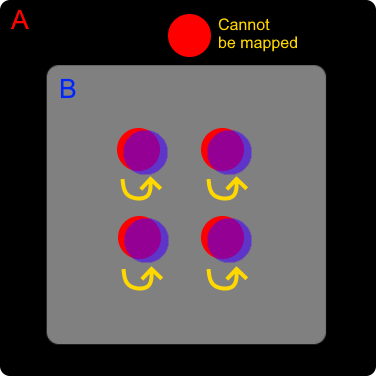
\includegraphics[scale=0.5]{Images/4.3.5.png}
\end{figure}

{ \color{red} Theorem 4.3.6: Infinite subsets of countable sets are countable } 

	\qquad An infinite subset E of a countably infinite set A is countably infinite.

{ \color{magenta} \underline{Proof} } 

	Let E $\subset$ A be an infinite subset.
	For every distinct $x_i$ $\in$ A, let x = \{ $x_1, x_2, ...$ \}.

	Let $n_1$ be smallest integer such that x$_{n_1}$ $\in$ E.

	Then let $n_2$ be the smallest integer where $n_2$ $>$ $n_1$ such that x$_{n_2}$ $\in$ E.

	Repeat the process to create sequence f(k) = \{ $x_{n_1}, x_{n_2}, ... , x_{n_k} , ...$ \}.

	Thus, there is a 1-1 correspondence between E and $\mathbb{Z}_+$ so
	E is countably infinite.

\begin{figure}[h]
	\centering
	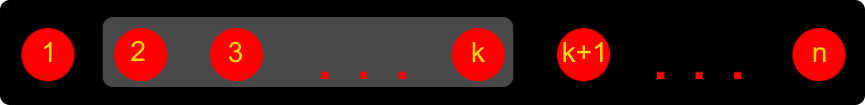
\includegraphics[scale=0.5]{Images/4.3.6.png}
\end{figure}





